% Author = warrior
% Date = 26/5/21

% Definitionsprojectestructure

%\documentclass{article}

% Links
% https://latex-tutorial.com/tutorials/
% https://robjhyndman.com/hyndsight/indexing-in-latex/
% https://es.overleaf.com/learn/latex/Headers_and_footers
% https://www.overleaf.com/learn/latex/Sections_and_chapters
% https://es.overleaf.com/learn/latex/Headers_and_footers

% Examples
% http://diposit.ub.edu/dspace/bitstream/2445/66890/2/memoria.pdf

% Vars

\newcommand\email{filter.oriol@gmail.com}
\newcommand\projectname{Online Shop Structure}


%\title{Online Shop Structure}
\title{\projectname}
%\date{26/05/2021}
\date{\today}
\author{Oriol Filter Anson\\\email}

% Preamble
\documentclass[11pt]{article}
%\makeindex

% Packages
\usepackage{amsmath}
\usepackage{lipsum}
\usepackage{graphicx}
\graphicspath{ {./images/} }
\usepackage[utf8]{inputenc}
\usepackage[english]{babel}
\usepackage{fancyhdr}
\usepackage{hyperref}
\usepackage{lastpage}
\usepackage{tikz}
\usetikzlibrary{patterns}
\usepackage{bchart}


%Includes
\usepackage{pgfplots}
\usepackage{listings}
\usepackage{xcolor}
\usepackage{verbatim}
\definecolor{codegreen}{rgb}{0,0.6,0}
\definecolor{codegray}{rgb}{0.5,0.5,0.5}
\definecolor{codepurple}{rgb}{0.58,0,0.82}
\definecolor{backcolour}{rgb}{0.95,0.95,0.92}

\lstdefinestyle{mystyle}{
    backgroundcolor=\color{backcolour},
    commentstyle=\color{codegreen},
    keywordstyle=\color{magenta},
    numberstyle=\tiny\color{codegray},
    stringstyle=\color{codepurple},
    basicstyle=\ttfamily\footnotesize,
    breakatwhitespace=false,
    breaklines=true,
    captionpos=b,
    keepspaces=true,
    numbers=left,
    numbersep=5pt,
    showspaces=false,
    showstringspaces=false,
    showtabs=false,
    tabsize=2
}





\newcommand\YAMLcolonstyle{\color{red}\mdseries}
\newcommand\YAMLkeystyle{\color{black}\bfseries}
\newcommand\YAMLvaluestyle{\color{blue}\mdseries}

\makeatletter

% here is a macro expanding to the name of the language
% (handy if you decide to change it further down the road)
\newcommand\language@yaml{yaml}

\expandafter\expandafter\expandafter\lstdefinelanguage
\expandafter{\language@yaml}
{
    keywords={true,false,null,y,n},
    keywordstyle=\color{darkgray}\bfseries,
    basicstyle=\YAMLkeystyle,                                 % assuming a key comes first
    sensitive=false,
    comment=[l]{\#},
    morecomment=[s]{/*}{*/},
    commentstyle=\color{purple}\ttfamily,
    stringstyle=\YAMLvaluestyle\ttfamily,
    moredelim=[l][\color{orange}]{\&},
    moredelim=[l][\color{magenta}]{*},
    moredelim=**[il][\YAMLcolonstyle{:}\YAMLvaluestyle]{:},   % switch to value style at :
    morestring=[b]',
    morestring=[b]",
    literate =    {---}{{\ProcessThreeDashes}}3
        {>}{{\textcolor{red}\textgreater}}1
        {|}{{\textcolor{red}\textbar}}1
        {\ -\ }{{\mdseries\ -\ }}3,
}

% switch to key style at EOL
\lst@AddToHook{EveryLine}{\ifx\lst@language\language@yaml\YAMLkeystyle\fi}
\makeatother

\newcommand\ProcessThreeDashes{\llap{\color{cyan}\mdseries-{-}-}}


\lstset{style=mystyle}

\pagestyle{fancy}
\fancyhf{}

\hypersetup{
    colorlinks=true,
    linkcolor=blue,
    filecolor=magenta,
    urlcolor=cyan,
    pdftitle={Overleaf Example},
%    pdfpagemode=FullScreen,
}

%https://github.com/marekaf/docker-lstlisting

\usepackage{listingsutf8}

\lstdefinelanguage{docker}{
  keywords={FROM, RUN, COPY, ADD, ENTRYPOINT, CMD,  ENV, ARG, WORKDIR, EXPOSE, LABEL, USER, VOLUME, STOPSIGNAL, ONBUILD, MAINTAINER},
  keywordstyle=\color{blue}\bfseries,
  identifierstyle=\color{black},
  sensitive=false,
  comment=[l]{\#},
  commentstyle=\color{purple}\ttfamily,
  stringstyle=\color{red}\ttfamily,
  morestring=[b]',
  morestring=[b]"
}

\lstdefinelanguage{docker-compose}{
  keywords={image, environment, ports, container_name, ports, volumes, links},
  keywordstyle=\color{blue}\bfseries,
  identifierstyle=\color{black},
  sensitive=false,
  comment=[l]{\#},
  commentstyle=\color{purple}\ttfamily,
  stringstyle=\color{red}\ttfamily,
  morestring=[b]',
  morestring=[b]"
}
\lstdefinelanguage{docker-compose-2}{
  keywords={version, volumes, services},
  keywordstyle=\color{blue}\bfseries,
  keywords=[2]{image, environment, ports, container_name, ports, links, build},
  keywordstyle=[2]\color{olive}\bfseries,
  identifierstyle=\color{black},
  sensitive=false,
  comment=[l]{\#},
  commentstyle=\color{purple}\ttfamily,
  stringstyle=\color{red}\ttfamily,
  morestring=[b]',
  morestring=[b]"
}

\lstset{basicstyle=\ttfamily,
  showstringspaces=false,
  commentstyle=\color{red},
  keywordstyle=\color{blue},
  inputencoding=utf8,
  extendedchars=true
}



%conf 1
\rfoot{Page \thepage \hspace{1pt} of~\pageref{LastPage}}
\lhead{\projectname}
\rhead{\email}
%conf 2
%\rhead{Page \thepage \hspace{1pt} of \pageref{LastPage}}
%\lfoot{\email}



% Document
\makeindex
\begin{document}
%    Tittle
    \clearpage
    \maketitle
    
\includegraphics[scale=1.5]{favicon}
    \thispagestyle{empty}

    \newpage
%    Index
    \tableofcontents{}
    \thispagestyle{empty}

    \newpage
%    Introduction
    \setcounter{page}{1}
    \section{Introduction}\label{sec:introduction}
            This section will make a resume about what's this project about, commend which where the motivation that bring
        me to carry on this project, how to implement it and use it, alongside with how to modify its behaviour.
        With the intention to make reader able to implement and configure it at its desire following simple and
        concise steps while providing a deep understanding of the followed actions.

    \newpage
%    Description
    \subsection{Description}\label{subsec:Description}

        This project is intended to facilitate implementing an online shop with a base infrastructure.
        Offering the capability of:
        \begin{itemize}
            \item Infrastructure based on dockers.
            \item Default web with simple configuration.
            \item Defined database structure.
            \item Backup automation to a local drive or remote server.
            \item Automatic error management among the web-database relation limiting the occurrence of errors.
        \end{itemize}

%    Motivation
    \subsection{Motivation}\label{subsec:Motivation}

        The motivation behind this project, was mainly finding an excuse in order to use different technologies and
        try to combine them, doing something that gives me a deeper understanding of the technologies and tools used.

%    Keywords
    \subsection{Keywords}\label{subsec:Keyords}

    PHP, PDO, Docker, Docker-compose, Dockerfile, Network, Api, Security, Infrastructure, Web, Nginx, Server, Portainer,
    Deploy, Swarm, LaTeX, Yaml, JSON, SSL, Certificates, SSH, Key, Users, Passwords, PostgreSQL, Stack, Groups, Shop,
    Online, Environment, Backups, Motorisation, Script, Bash, Shell, Git, Markdown, HTML, JavaScript, AJAX, Regex,
    Automation, Postgres, Database, HTTP, HTTPS, Client, Server, Crontab.


    \newpage
%    Main objective
    \subsection{Main Objective}\label{subsec:MainObjective}

        The main objective that bring me to build this project, was acquiring a deeper understanding about database
        management while providing a secure interface for its users in order to interact with its accounts without
        affecting at the response time from the client petitions, focused on the information minimization required for
        the user, and its security while using our services.
        Another topic that woke curiosity on me, was about regarding how API worked since neither knew how to implement
        nor interact with them, and meanwhile.

    \newpage
%    Secondary objective
    \subsection{Secondary Objectives}\label{subsec:SecondaryObjective}

        Meanwhile wasn't something that had on mind during the start of the project, it's something that built during
        the production of it, which was the desire of improve past knowledge and learn about new tools, familiarizing
        myself with its different applications and its possibilities.

        Some of them are:
        \begin{itemize}
            \item Dockerfiles and the production of new images.
            \item Github, and how to keep track of a project and its updates.
            \item PDO and how facilitates updating our database system without the need of updating the code of our
            existing pages.
        \end{itemize}


    \newpage


    \newpage
%    Secondary objective
    \subsection{Reasons}\label{subsec:Reasons}
        \subsubsection[PHP]{PHP}

        \begin{center}
            
\includegraphics[scale=0.3]{logo_php}
        \end{center}
        \begin{flushleft}
        The main reason I decided to use PHP over any other technology, was its actual usage among the world, which,
        taking a look at this graph, we can observe that its usage it's almost an 80\%, which confirms that even if there
        are upcoming technologies, PHP will keep there for a long time, so was a good idea familiarize myself with that
        language.
        \end{flushleft}

        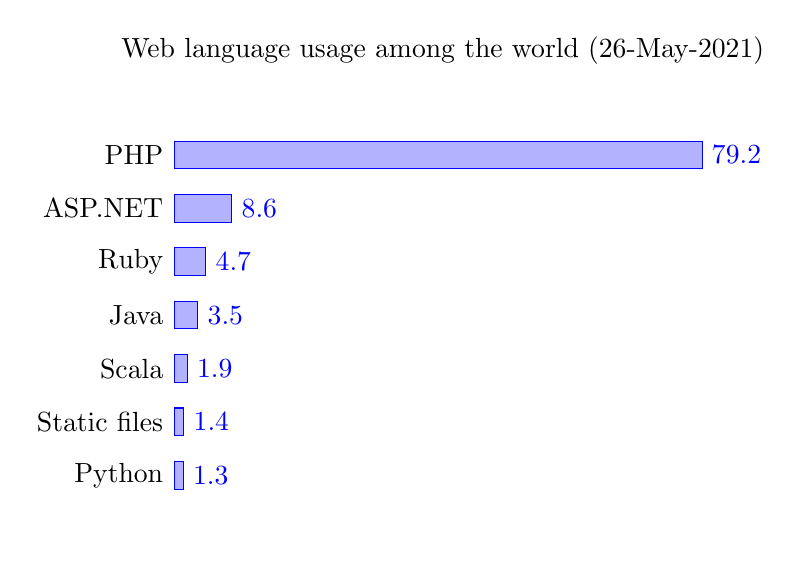
\begin{tikzpicture}
            \begin{axis}[title  = Web language usage among the world (26-May-2021),
                xbar,
                y axis line style = { opacity = 0 },
                axis x line       = none,
                tickwidth         = 0pt,
                ytick             = data,
                enlarge y limits  = 0.2,
                enlarge x limits  = 0.02,
                symbolic y coords = {Python, Static files, Scala, Java, Ruby, ASP.NET,  PHP},
                nodes near coords,
            ]
                \addplot coordinates { (79.2,PHP)         (8.6,ASP.NET)
                (4.7,Ruby)  (3.5,Java) (1.9,Scala) (1.4,Static files) (1.3,Python) };
            \end{axis}
        \end{tikzpicture}

        \url{https://w3techs.com/technologies/overview/programming_language}

        \subsubsection[Docker]{Docker}

        \begin{center}
            
\includegraphics[scale=0.3]{logo_docker}
        \end{center}

        \begin{flushleft}
            Regarding the docker decision, there wasn't much to think about, since docker is a modern technology which I
            already knew the bases, making it easier to pick up and start working earlier.
        \end{flushleft}

        \subsubsection[Docker-compose]{DockerCompose}

        \begin{center}
            
\includegraphics[scale=0.4]{logo_docker_compose}
        \end{center}

        \begin{flushleft}
            This tool facilitates deploying services on a server, while also being able to scalate the services or
            deploy them in a swarm, so there was no excuse to avoid its usage.
        \end{flushleft}

        \newpage
        \subsubsection[Portainer]{Portainer}

        \begin{center}
            
\includegraphics[scale=0.2]{logo_docker_portainer}
        \end{center}

        \begin{flushleft}
            Taking a look at different monitoring tools, decided to use docker portainer mainly by it's fast set-up.
            While still being up to the tasks demanded, which consist in monitoring and managing.
        \end{flushleft}

        \subsubsection[GitHub]{GitHub}

        \begin{center}
            
\includegraphics[scale=0.045]{logo_github}
        \end{center}

        \begin{flushleft}
            On the other hand, I decided to use GitHub to store the project mainly due having a basic understanding of how
            the tools work, since there are multiple tools that suits the same function, felt like that was the right decision.
        \end{flushleft}



        \newpage
        \subsubsection[PostgreSQL]{PostgresSQL}

        \begin{center}
            
\includegraphics[scale=0.3]{logo_postgresql}
        \end{center}

        \begin{flushleft}
            Meanwhile the web language was picked based on its global usage, I personally already have experience with
            Oracle, MySQL, MariaDB and MongoDB, so in order to try a different technology, I decided to use PostgreSQL,
            since it suited my needs while also learning a new database, yet, its position among the ranking, made the
            decision easier to take.
        \end{flushleft}

        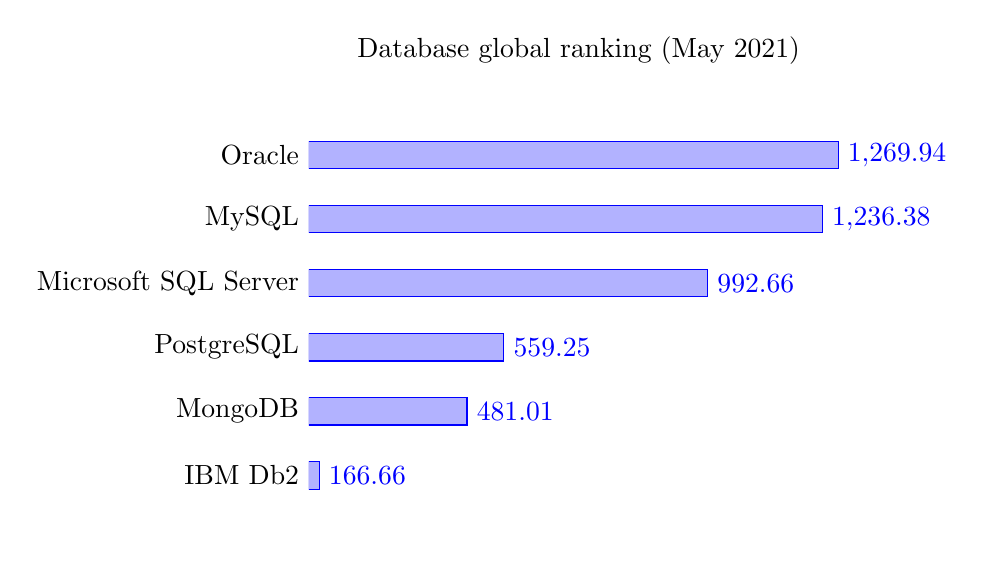
\begin{tikzpicture}
            \begin{axis}[title  = Database global ranking (May 2021),
            xbar,
            y axis line style = { opacity = 0 },
            axis x line       = none,
            tickwidth         = 0pt,
            ytick             = data,
            enlarge y limits  = 0.2,
            enlarge x limits  = 0.02,
            symbolic y coords = {IBM Db2, MongoDB, PostgreSQL, Microsoft SQL Server, MySQL,  Oracle},
            nodes near coords,
            ]
            \addplot coordinates { (1269.94,Oracle)         (1236.38,MySQL)
            (992.66 ,Microsoft SQL Server)  (559.25,PostgreSQL) (481.01,MongoDB) (166.66,IBM Db2) };
            \end{axis}
         \end{tikzpicture}

        \url{https://db-engines.com/en/ranking}

        \subsubsection[Nginx]{Nginx}

        \begin{center}
            
\includegraphics[scale=0.3]{logo_nginx}
        \end{center}
        \begin{flushleft}
            So far, being the main two options Apache and Nginx, I was quite limited when it came to variety,
            and yet, both suit its job very well, yet, due its minor differences, decided to use Nginx instead of Apache,
            since its less resource hungry while being more configurable-wise.
        \end{flushleft}

        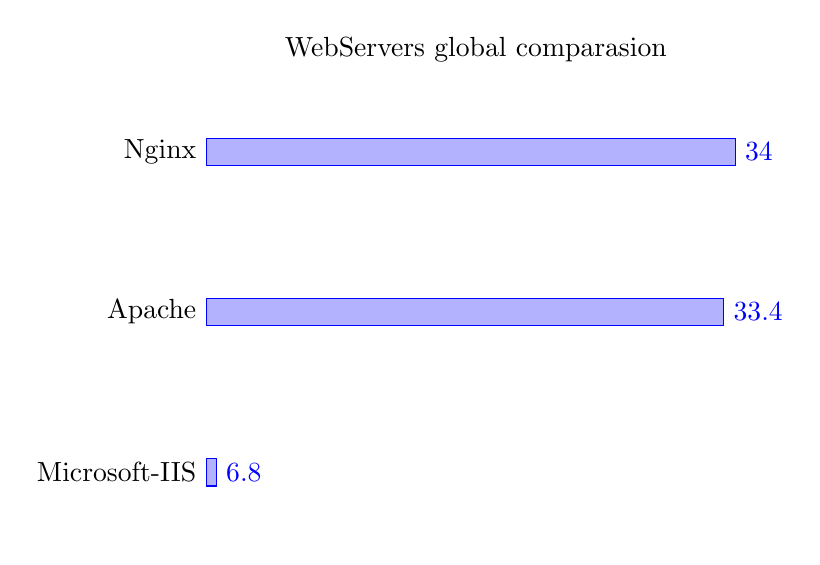
\begin{tikzpicture}
            \begin{axis}[title  = WebServers global comparasion,
            xbar,
            y axis line style = { opacity = 0 },
            axis x line       = none,
            tickwidth         = 0pt,
            ytick             = data,
            enlarge y limits  = 0.2,
            enlarge x limits  = 0.02,
            symbolic y coords = {Microsoft-IIS, Apache, Nginx},
            nodes near coords,
            ]
            \addplot coordinates { (34.0,Nginx) (33.4,Apache) (6.8 ,Microsoft-IIS)};
            \end{axis}
        \end{tikzpicture}

        \begin{flushleft}
            \url{https://w3techs.com/technologies/comparison/ws-apache,ws-microsoftiis,ws-nginx}
        \end{flushleft}

%    Project structure

    \newpage
%    Demo
    \section{Demo}\label{sec:Demo}
    \subsection[Main Page]{Main Page}\label{subsec:main-page}
\begin{center}
    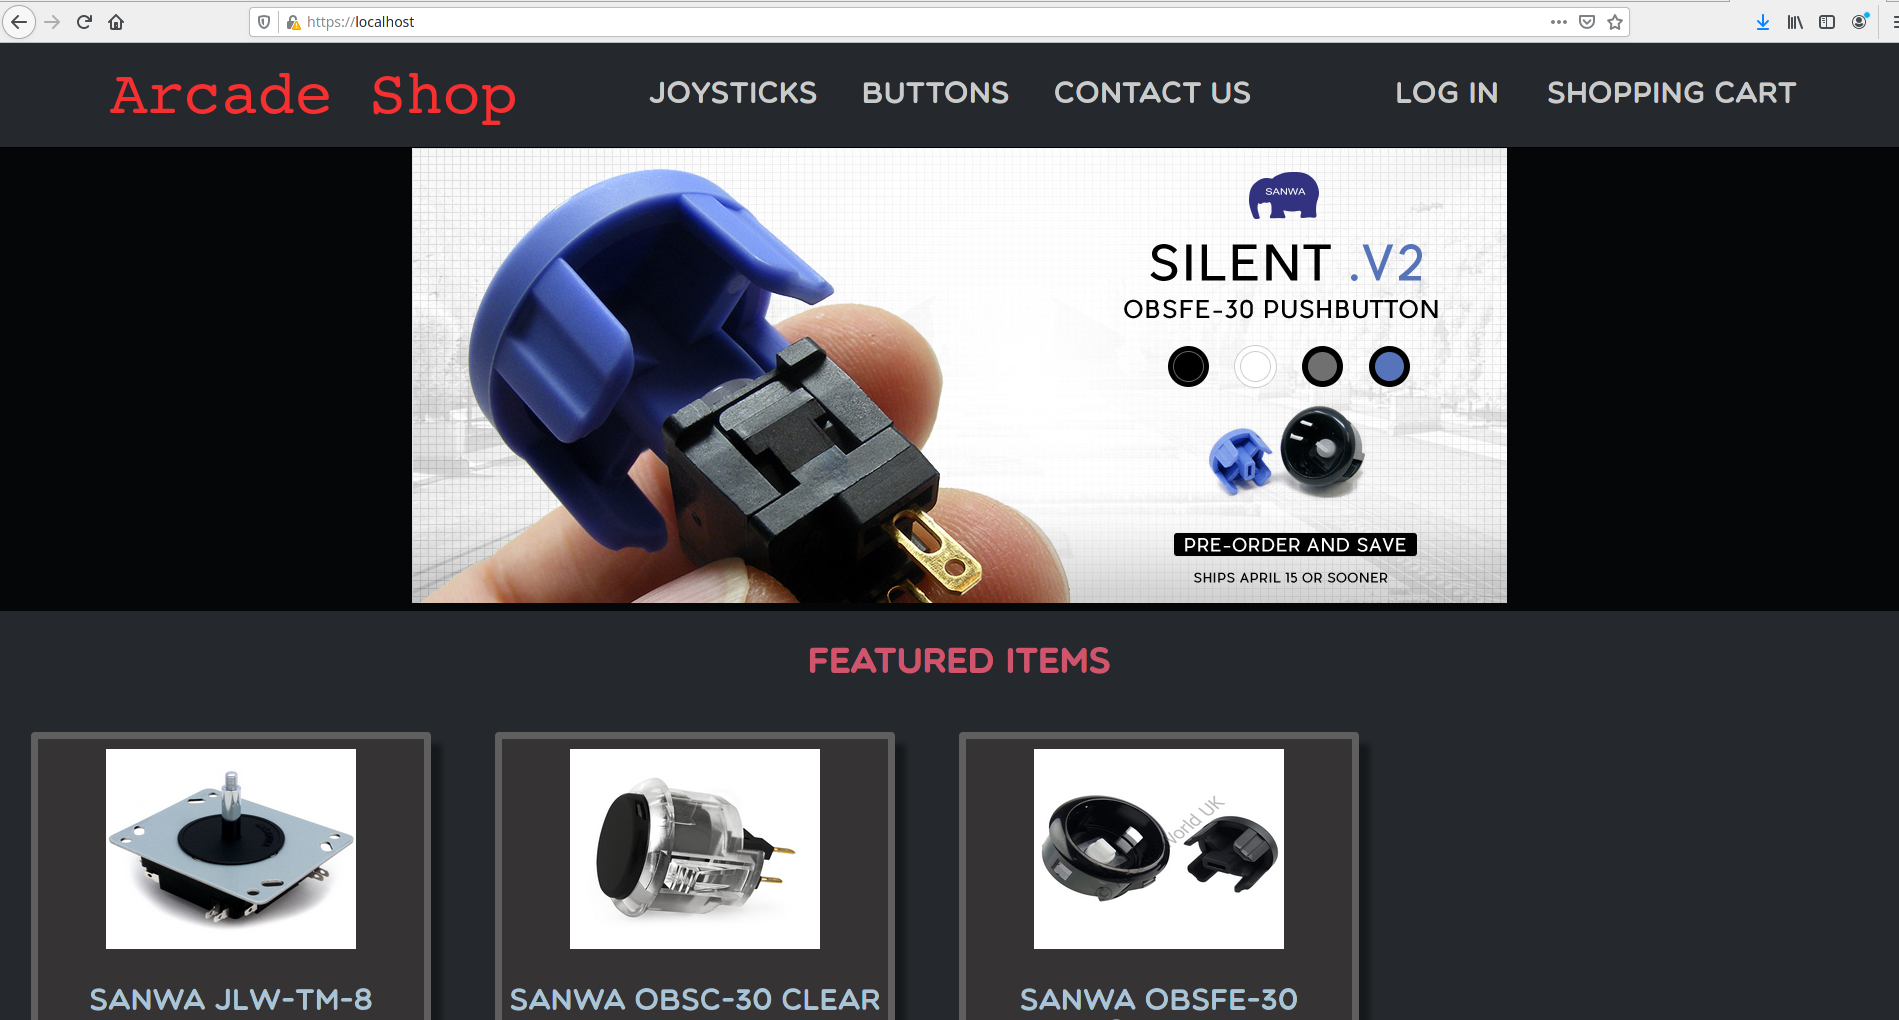
\includegraphics[scale=0.3]{demo_index}
\end{center}
\begin{flushleft}
    A simple view of the menu with different menus available, and a product showcase.
\end{flushleft}

\subsection[Registration Success Testing]{Registration Success Testing}\label{subsec:registration-success-testing}
\begin{center}
    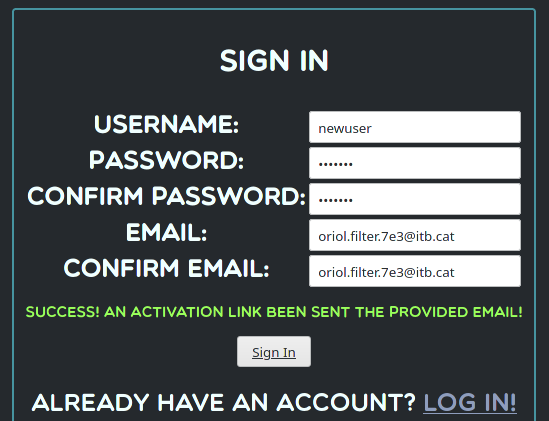
\includegraphics[scale=0.8]{demo_registration_success}
\end{center}
\begin{flushleft}
    We are able to receive responses from the server without the need of updating the page, in this case we were able to succeed in our registration.
\end{flushleft}

\subsection[Registration Fail Testing]{Registration Fail Testing}\label{subsec:registration-fail-testing}
\begin{center}
    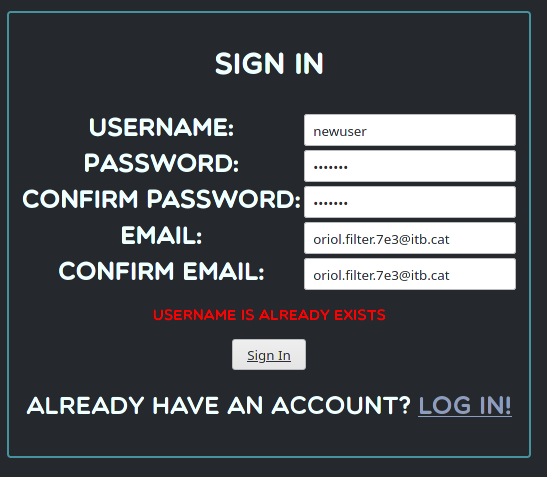
\includegraphics[scale=0.8]{demo_registration_failed}
\end{center}
\begin{flushleft}
    Since our user was already registered we receive a error response.
\end{flushleft}

\subsection[Login Unactivated Account Fail Testing]{Login Unactivated Account Fail Testing}\label{subsec:login-unactivated-account-fail-testing}
\begin{center}
    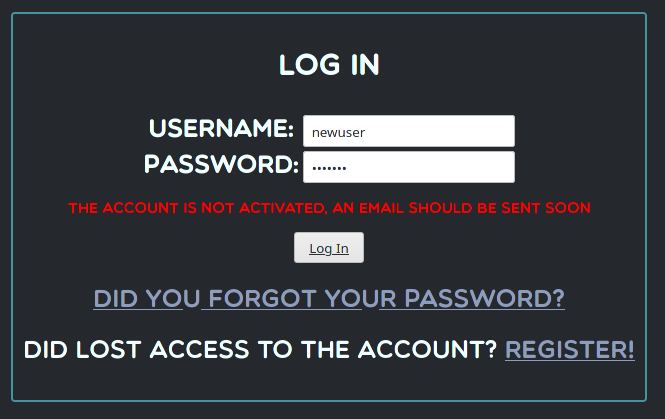
\includegraphics[scale=0.8]{demo_login_failed_unactivated}
\end{center}
\begin{flushleft}
    In order to activate our account, we need to activate our account via the received email.
\end{flushleft}

\subsection[Received email Testing]{Received email Testing}\label{subsec:received-email-testing}
\begin{center}
    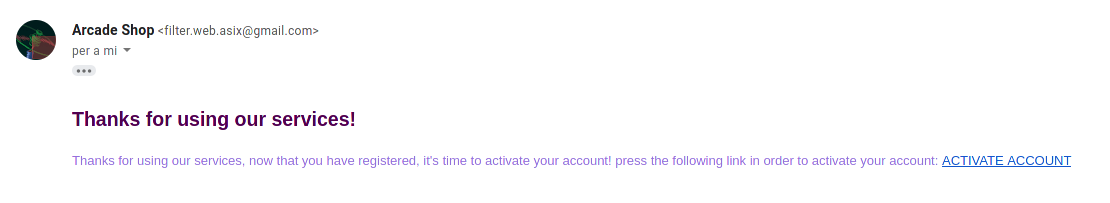
\includegraphics[scale=0.5]{demo_received_email}
\end{center}
\begin{flushleft}
    As expected, we are able to receive a mail to our given email.
\end{flushleft}

\subsection[Activate Account Succeed Testing]{Activate Account Succeed Testing}\label{subsec:activate-account-succeed-testing}
\begin{center}
    
\includegraphics[scale=0.8]{demo_activate_account_succeed}
\end{center}
\begin{flushleft}
    Once we open the link given by the server through the mail, we are able to activate our account.
\end{flushleft}

\subsection[Login Success Testing]{Login Success Testing}\label{subsec:login-success-testing}
\begin{center}
    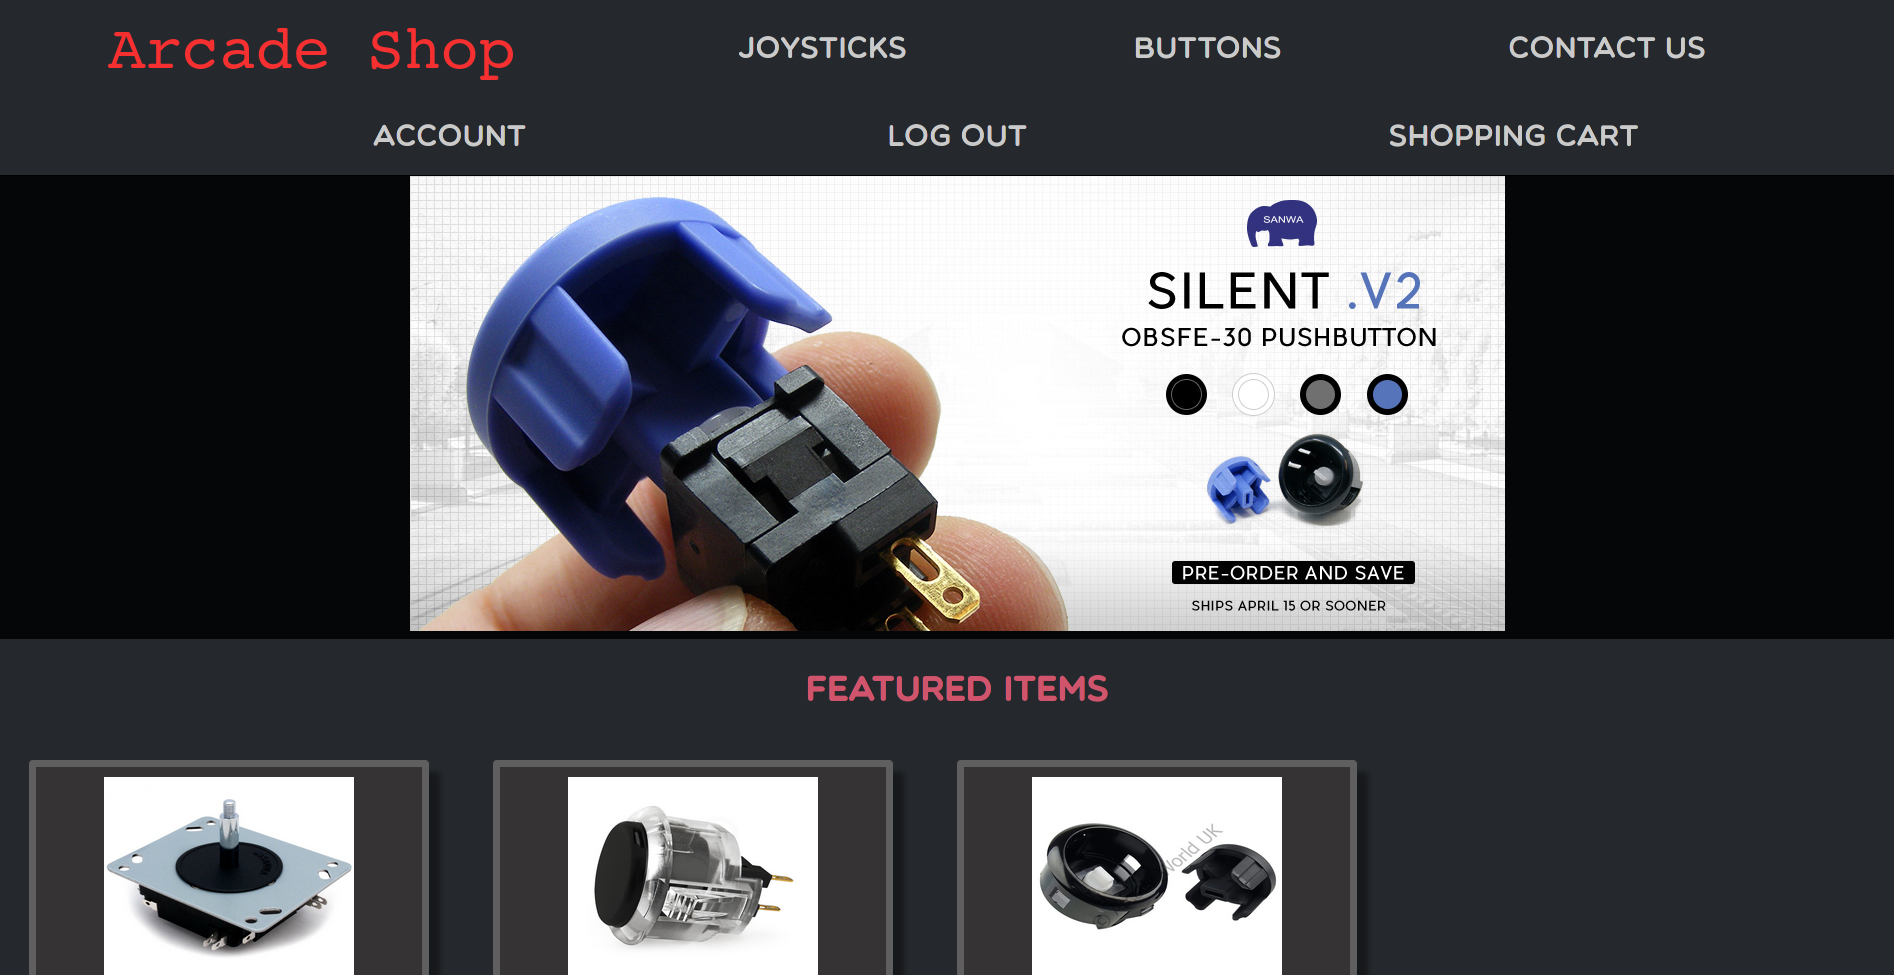
\includegraphics[scale=0.3]{demo_login_succeed}
\end{center}
\begin{flushleft}
    Once we have our account activated, we are able to login correctly, and afterwards we are redirected to the main
    menu, as a proof we can see how the menu it's quite different compared with when we didn't log in.
\end{flushleft}

\subsection[Add Shipping Address Fail Testing ]{Add Shipping Address Fail Testing}\label{subsec:add-shipping-address-fail-testing}
\begin{center}
    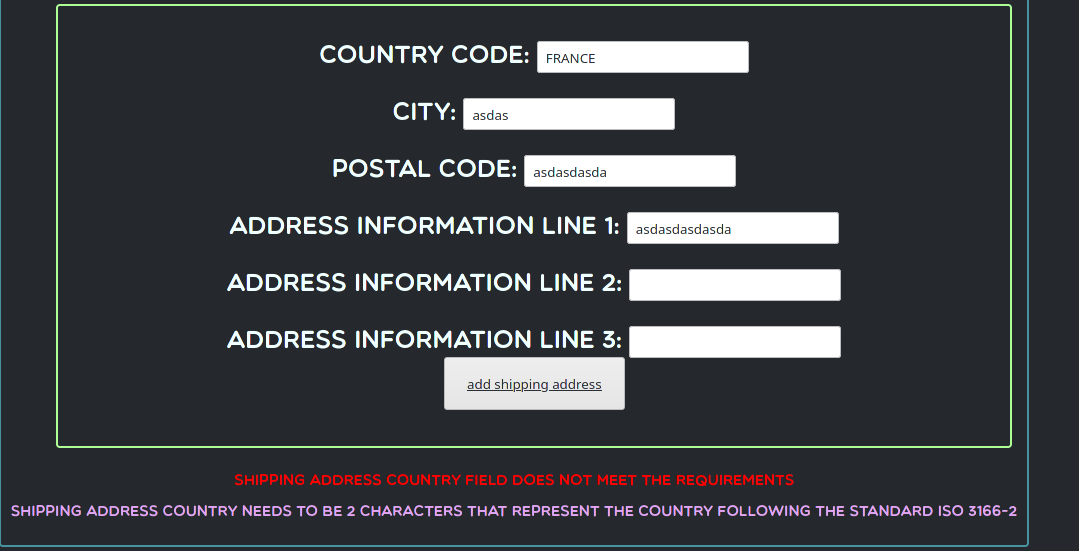
\includegraphics[scale=0.5]{demo_shipping_address_error}
\end{center}
\begin{flushleft}
    Since our country code doesn't consist of 2 characters, it returns error.
\end{flushleft}

\subsection[Add Shipping Address Success Testing ]{Add Shipping Address Success Testing}\label{subsec:add-shipping-address-success-testing}
\begin{center}
    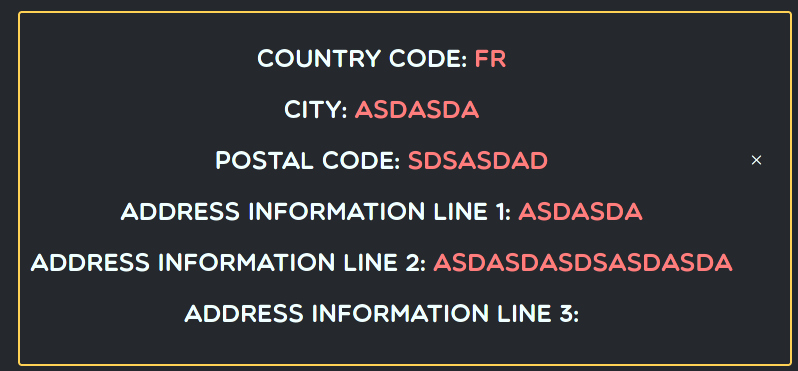
\includegraphics[scale=0.6]{demo_shipping_address_succeed}
\end{center}
\begin{flushleft}
    Once we respect the criteria from the fields, we are able to upload our payment method.
\end{flushleft}

\subsection[Remove Shipping Address Success Testing ]{Remove Shipping Address Success Testing}\label{subsec:remove-shipping-address-success-testing}
\begin{center}
    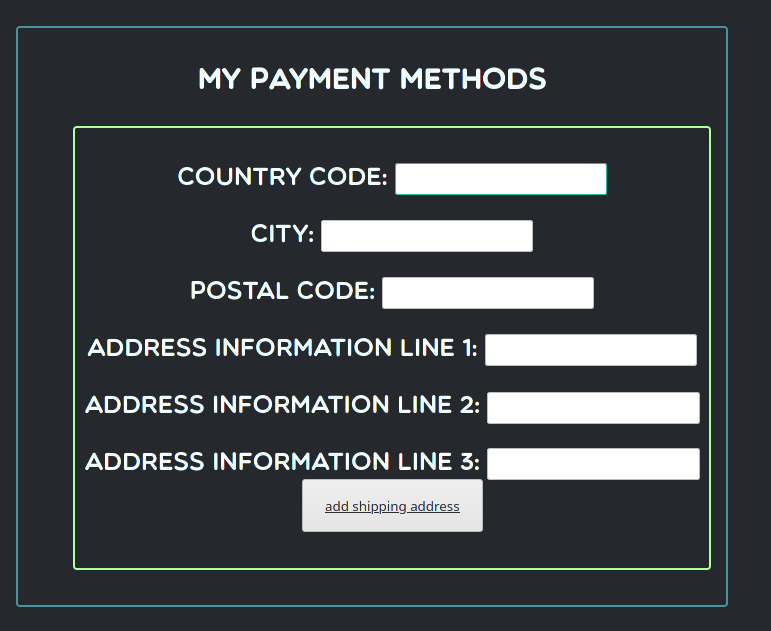
\includegraphics[scale=0.6]{demo_shipping_address_delete_succeed}
\end{center}
\begin{flushleft}
    Deleted the created entries without issues.
\end{flushleft}

\subsection[Cookies Testing]{Cookies Testing}\label{subsec:cookies-testing}
\begin{center}
    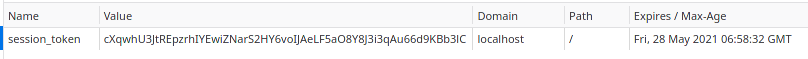
\includegraphics[scale=0.6]{demo_cookies}
\end{center}
\begin{flushleft}
    Checking the cookies, we can see our session token.
\end{flushleft}



    \newpage
%    Docker configuration
    \section{Docker Configuration}\label{sec:DockerConfiguration}
        \subsection{Docker Network Scheme}\label{subsec:ProjectNetworkScheme}
    \begin{center}
    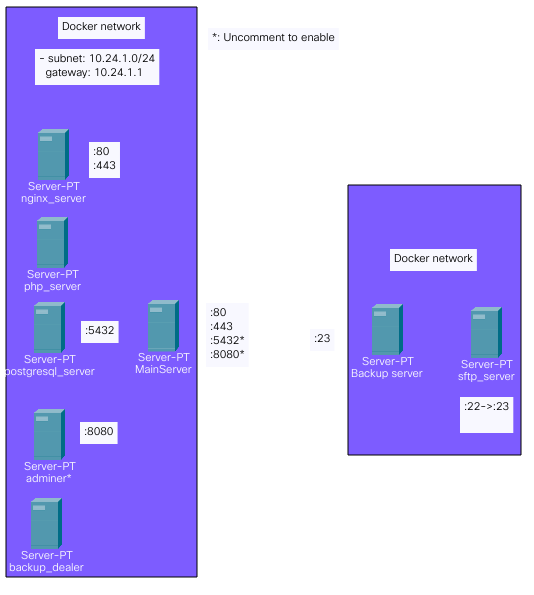
\includegraphics[scale=0.8]{NetworkDistribution}
    \end{center}
    \newpage

    \subsection{Docker Distribution Explanation}\label{subsec:dockernetworkexplanation}
    \begin{flushleft}
        As mentioned previously, the services are distributed in two servers, yet, the second one (the backup server),
        could be removed and store the backups locally, moving the \textbf{sftp} service to the main server, or, through
        \textbf{docker} using a volume or directory binding, but even if it's possible, it's recommended to do the backups in a
        different server as a security measure in case the main server get compromised.
    \end{flushleft}

    \begin{flushleft}
        Taking a look in the main server, we can see that the docker machines are mainly distributed among a common network,
        while there still an \textbf{docker} machine hanging by himself, that's because this \textbf{docker} machine is
        used to generate backups periodically, so doesn't need to have access to another docker networks (unless we wanted to specifically upload
        the backups inside a docker-machine that resides inside a docker network, but we didn't have the need
        to publish the ports in the main server, which is not the actual scenario, nor likely to happen).
    \end{flushleft}


    \subsubsection[Nginx]{Nginx}
    \begin{flushleft}
        Having the ports 80 and 443 exposed in the server, its configuration forces the use of the port 443, redirecting
        the connections fo that port, that way in case of having an HTTP petition the client is forced to use a "secure"
        connection, or at least, a connection that uses SSL encrypting.
    \end{flushleft}
    \begin{flushleft}
        Also does use of a docker volume to store the logs.
    \end{flushleft}

    \subsubsection[PHP]{SFTP}
    \begin{flushleft}
        While this container doesn't do nothing by himself, either has ports exposed, it's linked to the nginx server, providing php support
        to that container, where all will store the backups.
    \end{flushleft}

    \subsubsection[Postgresql]{Postgresql}
    \begin{flushleft}
        PostgreSQL uses by default the port 5432 to connect to the databases, and while there could be some reasons to
        have it exposed, but since in this scenario we aren't making use of it, it's better to keep it closed, that way
        the connections are limited to the docker machines themselves.
    \end{flushleft}
    \begin{flushleft}
        The container does use of a volume so store its data.
    \end{flushleft}
    \newpage
    \subsubsection[Adminer]{Adminer}
    \begin{flushleft}
        Like previously mentioned, the ports from the database are not exposed, but, in case of needing a simple GUI
        access to them, this can be arranged by using the adminer docker, which provides a web-database management,
        and since it's in the same docker network than the postgresql database, we can have access to it without having
        to expose the ports.
        The active configuration allows you to access the service using the port 8080.
    \end{flushleft}

    \subsubsection[Portainer]{Portainer}
    \begin{flushleft}
        To provide easy access to monitor and control the docker volumes, have decided to implement \textbf{Portainer}
        to the docker network, allowing the users to access to it using the port 9000.
    \end{flushleft}


    \subsubsection[Backup\_dealer]{BackupDealer}
    \begin{flushleft}
       Like mentioned previously, this machine is used to periodically do backups of the desired volumes or directories,
       to a local volume or directory, or to a remote server.
    \end{flushleft}

    \subsubsection[SFTP]{SFTP}
    \begin{flushleft}
        Observing the schema, we can see that the port 22 is being forwarded to the port 23, and publishing it, that's
        to avoid a port overlap with the default SSH port configuration.
        This container stores the backups in a volume named "backups\_volume".
    \end{flushleft}

    \newpage
    \subsection[Main Server Docker Configuration]{MainServerDockerConfiguration}\label{subsec:mainserverdockerconfiguration}
    \subsubsection[Main Server Docker-Compose]{Main Server DockerCompose}
    \lstinputlisting[language=Docker-compose,label={lst:MainDockerCompose}]{../docker-compose.yml}
%    \paragraph{docker-compose.yml} this file contains the services for the main server.

    \newpage
    \begin{flushleft}
        The main things worth to mention, besides the open ports which are already commented (yet again will be listed here),
        it's the restart policies and pointing out which services need to be build instead of using a raw image.
    \end{flushleft}
    \begin{enumerate}
        \item Networks:
            \begin{itemize}
                \item shop\_net:
                \begin{itemize}
                    \item nginx
                    \item php
                    \item adminer
                    \item postgresql
                \end{itemize}
                \item agent\_network:
                \begin{itemize}
                    \item portainer
                \end{itemize}
            \end{itemize}
        \item Volumes
            \begin{itemize}
                \item postgresql\_volume:
                \begin{itemize}
                      \item postgresql
                \end{itemize}
                \item portainer\_data:
                \begin{itemize}
                      \item portainer
                \end{itemize}
                \item nginx\_logs
                \begin{itemize}
                    \item nginx
                \end{itemize}
            \end{itemize}

    \end{enumerate}

    \begin{flushleft}
        The volume used to store the databases, it's mounted with "nocopy", to prevent data being copied data from that volume.
    \end{flushleft}
    \begin{flushleft}
        All the dockers have been configured to restart in case of failure, which means that unless they are stopped manually,
        they will always restart.
    \end{flushleft}


    \newpage
    \subsubsection[PHP Dockerfile]{PHP Dockerfile}
    \lstinputlisting[language=Docker,label={lst:PHPDockerfile}]{../Dockerfiles/php}
    \begin{flushleft}
        As listed in the Dockerfile, it's main (and only) function, is to install and enable PDO extension for PHP\@.
    \end{flushleft}

    \newpage
    \subsubsection[Postgresql Dockerfile]{Postgresql Dockerfile}
    \lstinputlisting[language=Docker,label={lst:PostgresqlDockerfile}]{../Dockerfiles/postgresql/Dockerfile}
    \begin{flushleft}
        This Dockerfile, instead of installing new packages to the image, it adds a script that will be called in case
        of not having data in the postgres folder, and also adds an SQL files that once executed, will be deleted
        from the machine in order to avoid security flaws.
    \end{flushleft}

    \newpage
    \subsubsection[Backup Dealer Docker-Compose]{Backup Dealer Docker-Compose}
    \lstinputlisting[language=Docker,label={lst:BackupDealerDockerCompose}]{../backup_dealer-compose.yml}
    \begin{flushleft}
        The main and only thing to point out, besides the fact that uses a Dockerfile, is that it's full of variables,
        this topic will be covered in the deployment section.
    \end{flushleft}

    \newpage
    \subsubsection[Backup Dealer Dockerfile]{Backup Dealer Dockerfile}
    \lstinputlisting[language=Docker,label={lst:BackupDealerlDockerfile}]{../Dockerfiles/backup_client/Dockerfile}
    \begin{flushleft}
        In comparison with the other 2 Dockerfiles which just fulfill one function, this one is more complex.
    \end{flushleft}
    \begin{flushleft}
        At the first Part it adds \textbf{Build} arguments and afterwards assign those arguments to environment variables
        to store its value in order to preserve it in future instances.

        Also initializes some variables with an empty value, which will require the user to specify them when using this docker.
    \end{flushleft}
    \begin{flushleft}
        Once the variables are set up, the Docker will install the packages required in order to accomplish its functions, which in this case the packages required are:
        \begin{itemize}
            \item : \textbf{Rsync} to generate backups from directories while keeping the permissions from the files.
            \item : \textbf{Tar} to compress the backups generated in order to reduce the size usage on the servers.
            \item : \textbf{Openssh} in order to be able to connect at the desired sftp server, so the backups can be
            item stored in a remote server.
            \item : \textbf{Keychain} so the backups can be fully automatized using certificates.
        \end{itemize}
    \end{flushleft}

    \begin{flushleft}
        Afterwards creates the default folders (based in the arguments given by the user, or using its default values),
        once it's done proceeds to add the file ".bashrc" with the content that will allow us to use a keychain avoiding the
        requirement of a password.
    \end{flushleft}
    \begin{flushleft}
        Finally, adds the "scripts" folder to the server.
    \end{flushleft}





    \newpage
%    Service Configuration
    \section{Services Configuration}\label{sec:ServicesConfiguration}
    \subsection{PostgreSQL Configuration}\label{subsec:postgresql-configuration}
\begin{flushleft}
    Currently, the database contains 2 databases.
    \begin{itemize}
        \item contact\_form
        \item shop
    \end{itemize}
    As a security feature, the login either by local or remote host, have enabled "SCRAM-SHA-256".
\end{flushleft}
\subsubsection[Contact database structure]{Contact database structure}
\begin{flushleft}
    As the name hints, this database is used to store the contact forms received using the contact page from the website.
    Yet, the database consists of one table.
\end{flushleft}

\begin{center}
    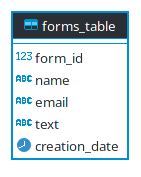
\includegraphics[scale=0.6]{DB_Table_Schema_Contact_FormV1}
\end{center}
\begin{center}
    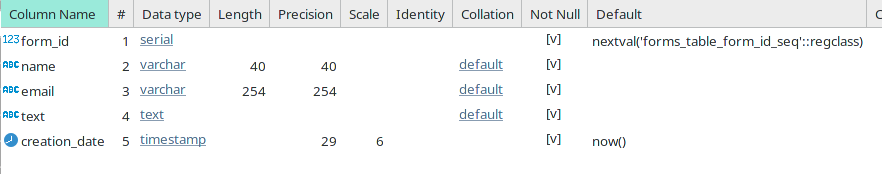
\includegraphics[scale=0.6]{DB_Table_Table_Contact_Form}
\end{center}

\begin{flushleft}
    As the name hints, this database is used to store the contact forms received using the contact page from the website.
    Yet, the database consists of one table.
\end{flushleft}
\begin{flushleft}
    It also contains a procedure called "insert\_form", which given the next information "\textit{(p\_name varchar,
    p\_email varchar, p\_text text)}", checks if the values are valid and in case of not being valid, will rise an error
    (more information in the Regex and Error List threads).
\end{flushleft}
\begin{flushleft}
    As a security measure, there been a user implemented using the next query:
    \lstinputlisting[language=SQL,label={lst:lstlisting}]{../Dockerfiles/postgresql/sources/contact_form_users.sql}
\end{flushleft}
\begin{flushleft}
    Taking a look at the query, we can observe that the first step is to revoke all the permissions in the database,
    that way we can ensure that all the users are limited to the options that we specifically gave.
\end{flushleft}


\newpage
\subsubsection[Shop database structure]{Shop database structure}
\begin{center}
%    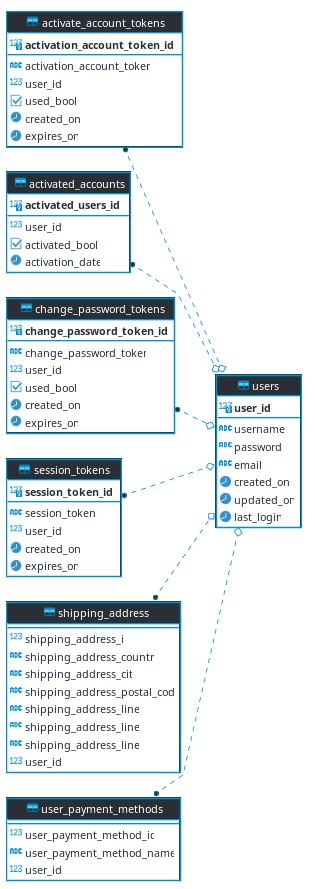
\includegraphics[scale=0.6]{DB_Table_Schema_ShopV1}
    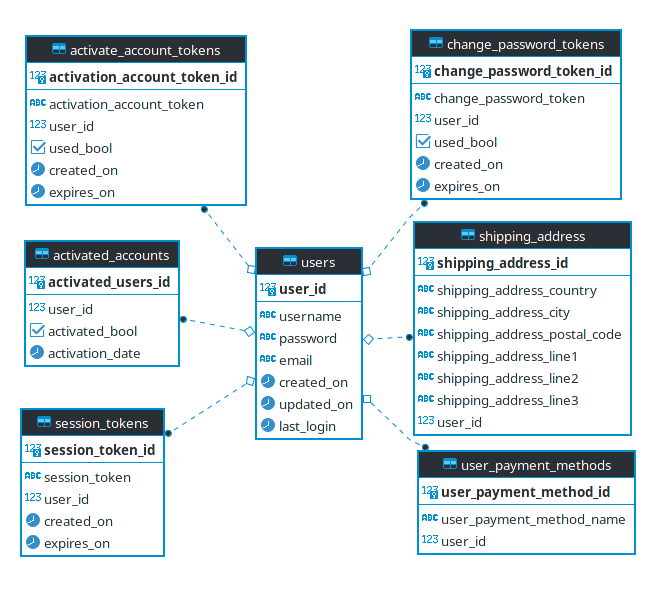
\includegraphics[scale=0.6]{DB_Table_Schema_ShopV4}
\end{center}
\begin{flushleft}
    Taking a look at the graph we can see how all the tables has a relation with the users table, bind by its user id.
    If we took a look at the queries used to create the tables, we could see how all would get deleted on cascade in case
    that the user was deleted.
    \url{https://github.com/OriolFilter/filterweb/blob/master/Dockerfiles/postgresql/sources/shop_skel.sql}
\end{flushleft}


\subsubsection[Plugins enabled]{Plugins enabled}
\begin{lstlisting}[language=SQL,label={lst:pgcrypto_enabling}]
CREATE EXTENSION if not exists pgcrypto;
\end{lstlisting}
\begin{flushleft}
    Pgcrypto was enabled in order to hash and salt the passwords, so the use critical information can be stored "securely".
\end{flushleft}

\newpage
\subsubsection[Data structure]{Data structure}
\begin{flushleft}
    \begin{itemize}
        \item Serial data (\_id values)
        \begin{itemize}
            \item Used to store data avoiding collisions while providing an identification point for the entry (used as a Primary Key).
        \end{itemize}
        \item Username
            \begin{itemize}
                \item Varchar of 20 length, still, it could be any length, even text, since how postgresql reserves memory,
                but in order to avoid issues during interactions with other applications, or, to facilitate upgrading to
                another Database System in the future (if it's needed), it's better to keep it sort of short.
                \begin{flushleft}
                    Usernames are checked by the next function: "function\_check\_user\_exists" returning a boolean, or
                    procedure "proc\_check\_user\_exists" raising an error in case the username already exists.
                \end{flushleft}
            \end{itemize}
        \item Password
        \begin{itemize}
            \item Varchar of 60 length since it's the length of a hashed value.
            \begin{flushleft}
                Passwords are hashed and use salt 8, while not providing any word to salt the value, being this one "randomized".
            \end{flushleft}
        \end{itemize}
        \item Email
        \begin{itemize}
            \item Varchar of 255 length since according to the next post, emails are actually unable to overcome that length.
            If in the future that changed, it could be easily modified.
            \begin{flushleft}
                \url{https://stackoverflow.com/questions/386294/what-is-the-maximum-length-of-a-valid-email-address}
            \end{flushleft}
        \end{itemize}
        \item created\_on - updated\_on - last\_login
        \begin{itemize}
            \item Stores a time stamp.
        \end{itemize}
        \item expires\_on
        \begin{itemize}

            \item Also stores a time stamp, but this one will also be used to check if the token for something (its function
            might depend on of which table is stored).
            By default  it's +30 minutes from its creation.
            \begin{flushleft}
            Used to check:
                \begin{itemize}
                    \item Login session is valid
                    \item Activate account token is valid
                    \item Update/Change password token is valid
                \end{itemize}
            \end{flushleft}
        \end{itemize}
        \item \_token values / varchar (200)
        \begin{itemize}
            \item Used to store randomized tokens.
            Like in the username or email fields, the value could ve easily modified if it was needed in the future.
        \end{itemize}
        \item shipping / payment methods data
        \begin{itemize}
            \item Mainly stored as a varchar, the length might vary depending on of the needs.
        \end{itemize}
    \end{itemize}
\end{flushleft}

\newpage
\subsubsection[Main functions]{Main functions}
\begin{flushleft}
    Like posteriorly will be shown with the error codes, postgresql it's intended to "break" (generate an error), in
    case something goes wrong.
    So it's mainly formed by procedures instead of functions, unless it's specifically required.

    \begin{itemize}
        \item  function return\_crypted\_pass(v\_txt varchar)
        \begin{itemize}
            \item Returns the hashed + salted (8) password using the function "crypt" (module "pgcrypto").
        \end{itemize}
        \item  procedure register\_user
        \begin{itemize}
            \item Registers the user with the values given, before inserting the values, checks that the values are valid.
        \end{itemize}
        \item  proc\_login\_session\_token
        \begin{itemize}
            \item Checks the given session token is valid, in case of being valid will enlarge its session 30 minutes from the moment,
            its used when the user loads a page.
        \end{itemize}
    \end{itemize}
\end{flushleft}


\newpage
\subsection{Data Validation}\label{subsec:data-validation}
\subsubsection[Regex]{Regex}

\begin{lstlisting}[language=yaml,label={lst:regexListing}]
PHP & JS:
    Registration:
        username: "^[a-zA-Z0-9_.+]{6,20}$"
        password: "^[a-zA-Z0-9$%.,?!@+_=-]{6,20}$"
        email:    "^[a-zA-Z0-9.!#$%&'*+/=?^_`{|}~-]+@[a-zA-Z10-9-]+\.+[a-zA-Z0-9-]+$"

    Contact form:
        name:  "^[\w0-9 ]{4,40}$"
        email: "^[a-zA-Z0-9.!#$%&'*+/=?^_`{|}~-]+@[a-zA-Z10-9-]+\.+[a-zA-Z0-9-]+$"
        text:  "^[\w\W]{20,255}$"

    Change password form:
        token: "^[a-zA-Z0-9]{60}$"

    Payment methods:
        name: '^[a-zA-Z0-9 ]{6,20}$'
        id: '^[0-9]+$'
    Shipping adress:
        Country code: '/^[a-zA-Z]{2}$/'
        id: '/^[0-9]+$/'
        postal code & city: '/^[\w\W]+$/' # Checks not empty
        address line 1: '/^[\w\W]{5,200}$/'
        address line 2 & 3 : "/^[\w\W]*$/" # A lie, doesn't checks nothing

POSTGRESQL:
    Contact form:
        name:  "^[\w0-9 ]{4,40}$"
        email: "^[a-zA-Z0-9.!#$%&'*+=?^_`{|}~-]+@[a-zA-Z10-9-]+\.[a-zA-Z0-9-]+$"
\end{lstlisting}

\subsubsection[Javascript]{Javascript}

\begin{flushleft}
    Uses Regex and default java functions in order to check if the fields are valid, yet it doesn't really look at specific stuff.
\end{flushleft}

\begin{flushleft}
    Uses Ajax when receiving a response from the server, so can format a response for the user.
\end{flushleft}

\subsubsection[PostgreSQL]{PostgreSQL}

\begin{flushleft}
    Uses functions and procedures in order to detect errors, alongside with Regex.
\end{flushleft}

\subsubsection[PHP]{PHP}
\begin{flushleft}
    Uses functions and procedures in order to detect errors, alongside with Regex.
    PHP uses the errors captured to form a response for the client.
\end{flushleft}

\subsection{Error Thread}\label{subsec:error-thread}
\subsubsection{Notes}\label{subsubsec:notes}
\begin{flushleft}
    The errors are supposed to be handled by something, but not by postgresql (unless it's something specific), since
    there is no need of rollback/commit, due postgresql nature, that controls this automatically.
\end{flushleft}
\begin{flushleft}
    PHP and JavaScript uses these errors to format responses for the client based in the code received.
\end{flushleft}

\subsubsection{Error Codes}\label{subsubsec:error-codes}
\begin{lstlisting}[language=yaml,label={lst:errorListing}]
php & js:
    '0': 'Unknown error',

    '1': 'Success',

    '2': 'Missing field(s)',
    '2.1': 'Username field is missing',
    '2.2': 'Password field is missing',
    '2.3': 'Email field is missing',
    '2.4': 'Repeat password field is missing',
    '2.5': 'Repeat email field is missing',
    '2.6': 'Name field is missing',
    '2.7': 'Text field is missing',
    '2.8': 'Payment method name field is missing',
    '2.9': 'Payment method info field is missing',
    '2.10': 'Payment method id field is missing',
    '2.11': 'Shipping address fields topic',
    '2.11.1': 'Shipping address country field is missing',
    '2.11.2': 'Shipping address city field is missing',
    '2.11.3': 'Shipping address postal code field is missing',
    '2.11.4': 'Shipping address line 1 field is missing',
    '2.11.5': 'Shipping address id field is missing',

    '3': 'Requirements not achieved',
    '3.1': 'Username does not meet the requirements',
    '3.2': 'Password does not meet the requirements',
    '3.3': 'Email does not meet the requirements',
    '3.4': 'Name does not meet the requirements',
    '3.5': 'Text does not meet the requirements',
    '3.6': 'Payment method name does not meet the requirements',
    '3.7': 'Payment method info does not meet the requirements',
    '3.8': 'Payment method id does not meet the requirements', # It's a numeric value only
    '3.9': 'Shipping address fields topic',
    '3.9.1': 'Shipping address country field does not meet the requirements',
    '3.9.2': 'Shipping address city field does not meet the requirements',
    '3.9.3': 'Shipping address postal code field does not meet the requirements',
    '3.9.4': 'Shipping address line 1 field does not meet the requirements',
    '3.9.5': 'Shipping address line 2 field does not meet the requirements',
    '3.9.6': 'Shipping address line 3 field does not meet the requirements',
    '3.9.7': 'Shipping address id does not meet the requirements', # It's a numeric value only

    '4': 'Field matching',
    '4.1': 'Passwords don\'t match',
    '4.2': 'Emails don\'t match',

    '5': 'Client-Server errors',
    '5.1': 'There was a unknown error sending the data, please, try again bit later, if this error is consistent please contact an administrator.',
    '5.2': 'Server under maintenance, please, try again bit later.'

    '6': 'Database side error'
    '6.1': 'Data Insert errors',
    '6.1.1': 'Username is already exists',
    '6.1.2': 'Email is already exists',

    '6.2': 'Data Select errors',
    '6.2.1': 'Username not found',
    '6.2.2': 'User_id not found',
    '6.2.3': 'Email not found',
    '6.2.4': 'Token not found',
    '6.2.5': 'Payment method not found',
    '6.2.6': 'Shipping address not found',

    '6.3': 'Tokens',
    '6.3.1': 'Token not valid',
    '6.3.2': 'Token already used',
    '6.3.3': 'Token expired',
    '6.3.4': 'Token is null or empty',

    '6.4': 'Database connection error',
    '6.4.1': 'Error communicating to database',
    '6.4.2': 'Wrong credentials connecting to database',
    '6.4.3': 'The user don\'t has permission for the requested action(s)',

    '6.5': 'Functions error',
    '6.5.1': 'Error generating token',


    '7': 'Account related issues',
    '7.1': 'The account is not activated',
    '7.2': 'The account is already activated',
    '7.3': 'The account been banned',

    '8': 'PHP mailer issues',
    '8.1': 'Email couldn\'t be send',
    '8.2': 'Email address is missing',
    '8.3': 'Body is missing',
    '8.4': 'Subject is missing',

    '9': 'Invalid Credentials',

    '10': 'Product stuff',

    '11': 'User conf stuff',

    '11.2': 'Not valid payment method data'

    '12': 'Order Stuff'
postgresql:
  - 'Due postgresql not being able to use the same syntax as php and since the error codes seems easy to read using the syntax already done, it's been decided to leave the php and js codes as they, while using a similar (but valid) syntax for postgresql.'
  - 'P0000'
  - 'P + first number + second number +  last number'
  examples:
    - '7     :P7000'
    - '8.3   :P8300'
    - '6.4.4 :P6404'
    - '2.1   :P2100'
    - '2.10  :P2010'
\end{lstlisting}


    \newpage
%    Service deployment
    \section{Services Deployment}\label{sec:ServiceDeployment}
    \subsection{System requirements}\label{subsec:system-requirements}
\begin{flushleft}
    To install and configure the packages, a user with root access might be required, in case your system doesn't have the package
    "\textbf{sudo}", and your user be configured with it, consider swapping to the Root user.
\end{flushleft}

\begin{itemize}
    \item Access to internet
    \item Git
    \item Docker
    \item Docker-compose
\end{itemize}

\subsubsection{Git installation}
\paragraph{apt}
\begin{flushleft}
\begin{lstlisting}[language=bash,label={lst:apt-git}]
sudo apt-get update && sudo apt-get install git
\end{lstlisting}
\end{flushleft}

\paragraph{pacman}
\begin{flushleft}
\begin{lstlisting}[language=bash,label={lst:pacman-git}]
sudo pacman -Syu && sudo pacman -S git
\end{lstlisting}
\end{flushleft}

\paragraph{apk}
\begin{flushleft}
\begin{lstlisting}[language=bash,label={lst:apk-git}]
sudo apk update && sudo apk add --no-cache git
\end{lstlisting}
\end{flushleft}


\subsubsection{Docker installation}

\paragraph{apt}
\begin{flushleft}
\begin{lstlisting}[language=bash,label={lst:apt-docker}]
sudo apt-get update && sudo apt-get install docker-ce docker-ce-cli containerd.io
\end{lstlisting}
\end{flushleft}

\paragraph{pacman}
\begin{flushleft}
\begin{lstlisting}[language=bash,label={lst:pacman-docker}]
sudo pacman -Ss && sudo pacman -S docker
\end{lstlisting}
\end{flushleft}

\paragraph{apk}
\begin{flushleft}
\begin{lstlisting}[language=bash,label={lst:apk-docker}]
sudo apk update && sudo  apk add --no-cache docker
\end{lstlisting}
\end{flushleft}

\subsubsection{Docker configuration - allow user to use docker}
\begin{lstlisting}[language=bash,label={lst:add-group-docker}]
sudo usermod -a -G docker your_user
\end{lstlisting}

\subsubsection{Docker configuration - enable docker on boot}
\paragraph{service}
\begin{flushleft}
\begin{lstlisting}[language=bash,label={lst:service-docker}]
sudo service enable docker
\end{lstlisting}
\end{flushleft}

\paragraph{systemctl}
\begin{lstlisting}[language=bash,label={lst:systemctl-docker}]
sudo systemctl start
\end{lstlisting}

\paragraph{rc-update}
\begin{flushleft}
\begin{lstlisting}[language=bash,label={lst:rc-docker}]
sudo run rc-update add docker boot
\end{lstlisting}
\end{flushleft}

\subsubsection{Docker-Compose installation}
\paragraph{apt}
\begin{flushleft}
\begin{lstlisting}[language=bash,label={lst:apt-compose}]
sudo apt-get update && sudo apt-get install python3
sudo curl -L "https://github.com/docker/compose/releases/download/1.29.2/docker-compose-$(uname -s)-$(uname -m)" -o /usr/local/bin/docker-compose
sudo chmod +x /usr/local/bin/docker-compose
\end{lstlisting}
\end{flushleft}

\paragraph{pacman}
\begin{flushleft}
\begin{lstlisting}[language=bash,label={lst:pacman-compose}]
sudo pacman -Ss && sudo pacman -S python3
sudo curl -L "https://github.com/docker/compose/releases/download/1.29.2/docker-compose-$(uname -s)-$(uname -m)" -o /usr/local/bin/docker-compose
sudo chmod +x /usr/local/bin/docker-compose
\end{lstlisting}
\end{flushleft}

\paragraph{apk}
\begin{flushleft}
\begin{lstlisting}[language=bash,label={lst:apk-compose}]
sudo apk update && sudo  apk add --no-cache py-pip python3-dev libffi-dev openssl-dev gcc libc-dev rust cargo make
sudo curl -L "https://github.com/docker/compose/releases/download/1.29.2/docker-compose-$(uname -s)-$(uname -m)" -o /usr/local/bin/docker-compose
sudo chmod +x /usr/local/bin/docker-compose
\end{lstlisting}
\end{flushleft}


\subsubsection{Repository installation}\label{subsubsec:repo-installation}
\begin{flushleft}
    The only step is to clone the repository.
    \begin{flushleft}
        \textbf{git clone \url{\repoURL}}
    \end{flushleft}
\end{flushleft}




\subsection{Repository deployment minimal customization}\label{subsec:repo-customization}
\subsubsection[Main server deployment minimal customization]{Main server deployment minimal customization}
\lstinputlisting[language=bash, label={lst:main_env_file}]{../.env}
\begin{flushleft}
    The only to edit it's the \textbf{hostname}, since we need to replace it for our public/local \textbf{IP}
    or our \textbf{Domain Name}, in case we just wanted to test it, we could use "\textbf{localhost}".
\end{flushleft}

\newpage
\subsubsection[Backups client deployment minimal customization]{Backups client deployment minimal customization}
\begin{flushleft}
    \lstinputlisting[language=bash,label={lst:env_bk_pg}]{../bkcli_env_folder/.env_bk_pg}
    \lstinputlisting[language=bash,label={lst:env_bk_nx}]{../bkcli_env_folder/.env_bk_nx_logs}
    First we need to specify the \textbf{SFTHOST} for the \textbf{SFTP} server address, either the \textbf{IP} or the
    \textbf{Domain Name}, in this case, we can't use "localhost", in case we hosted the \textbf{SFTP} server in the same machine
    than the \textbf{bakcup\_dealer}, we need to specify our local \textbf{IP}.
\end{flushleft}

\subsubsection[Cron periodical backups minimal customization]{Cron periodical backups minimal customization}
\begin{flushleft}
    Once we have modified both \textbf{.env\_bk\_pg} and \textbf{.env\_bk.\_nx\_logs}, we need to execute the next command in order to do
    a backup every day.
    \begin{lstlisting}[language=bash,label={lst:insert_to_cron}]
echo "* * */1 * * $USER docker-compose -f $(pwd)/backup_dealer-compose.yml --env-file $(pwd)/bkcli_env_folder/.env_bk_pg up" | sudo tee -a  /etc/cron.d/docker_backups
echo "* * */1 * * $USER docker-compose -f $(pwd)/backup_dealer-compose.yml --env-file $(pwd)/bkcli_env_folder/.env_bk_ng_logs up"  | sudo tee -a  /etc/cron.d/docker_backups
    \end{lstlisting}
\end{flushleft}

\newpage
\subsubsection[Backups Server deployment minimal customization]{Backups Server deployment minimal customization}
\begin{flushleft}
    In case that we desire to host the server \textbf{SFTP} during the testing, we can skip this step.
\end{flushleft}

\begin{flushleft}
    The next step is copy the folder "backup\_server" to the device that we want to use as a backup server, this step
    isn't necessary if we already have a \textbf{SFTP} server, or we desire to do local backups(which isn't recommendable).

    To copy the folder to a remote server we can use the command:
\begin{lstlisting}[language=bash,label={lst:scp}]
scp -r ./backup_server <user>@<host>:~
\end{lstlisting}
\end{flushleft}

\subsection{Repository deployment booting services}\label{subsec:repository-deployment-booting-services}
\subsubsection[Main Server Service Booting]{Main Server Service Booting}
This can simply be done by executing the next command:
\begin{lstlisting}[language=bash,label={lst:compose-up}]
docker-compose build && docker-compose up
\end{lstlisting}

\subsubsection[Backup (Remote) Server Service Booting]{Backup (Remote) Server Service Booting}
\textit{Reminder that the server needs to fulfill the requirements.}
This can simply be done by executing the next command:
\begin{lstlisting}[language=bash,label={lst:compose-up-bk-remote}]
ssh <user>@<host> docker-compose -f backup_server/docker-compose.yml up -d
\end{lstlisting}

\subsubsection[Backup (Local) Server Service Booting]{Backup (Local) Server Service Booting}
This can simply be done by executing the next command:
\begin{lstlisting}[language=bash,label={lst:compose-up-bk-Local}]
docker-compose -f backup_server/docker-compose.yml up -d
\end{lstlisting}

\newpage
\subsection{Repository deployment further customization}\label{subsec:repository-deployment-further-customization}
\subsubsection[Custom SSL Keys]{Custom SSL Keys}
\begin{flushleft}
    In order to change the current certificates, you need to replace them for yours, the location of each certificate
    it's in the \textbf{docker-compose} document

    This applies for the \textbf{NGINX} and \textbf{SFTP} containers.
\end{flushleft}

\subsubsection[Custom Keychains]{Custom Keychains}
\paragraph{Requirements:} Keychain package installed.
\begin{flushleft}

    Once the requirements are fulfilled.
    We can proceed to generate the keychains.
    \begin{lstlisting}[label={lst:generating_keychain,language=bash}]
ssh-keygen -t rsa -b 2048 -f ./id_rsa
    \end{lstlisting}
\end{flushleft}
\begin{flushleft}
    Once we have created the keys, it's time to replace them, remember that the files need to be replaced in the local
    system AND the server in case the SFTP server is remote.
\end{flushleft}
\begin{flushleft}
    In case of modifying the path to the keys in the docker-compose file, remember that the \textbf{backup dealer} also
    makes use of these keys in order to login without need of password, so in case of changing its path, you need to do
    it in both files.
\end{flushleft}
%

\subsubsection[Adding more folders or modifying the current docker\_backup user]{Adding more folders or modifying the current docker\_backup user}
\begin{flushleft}
    In order to do this, we need to edit the file "\textit{users.conf}", located in the same folder as the \textbf{SFTP} server.
    \lstinputlisting[language=bash,label={lst:users.conf}]{../backup_server/users.conf}
    The file structure is:

\begin{lstlisting}[language=bash,label={lst:users.conf_hash_structure}]
USER:hashed_password:e:UID:GUID:folder_list
\end{lstlisting}
    In our case, since we don't need the user to have a password, since we are using keychains, we can just skip that field.
    \begin{lstlisting}[language=bash,label={lst:users.conf_structure}]
USER::UID:GUID:folder_list
    \end{lstlisting}
\end{flushleft}

\subsubsection[Deploying Custom Databases]{Deploying Custom Databases}
\begin{flushleft}
    In order to use/create our custom databases, we have 2 options, using a volume or directory that already has them
    created, or using the script that triggers if the directory "\textit{/data}" is empty, happen on mounting an empty
    volume, or the first time the container starts.
\end{flushleft}
\paragraph{Script/Building explanation}
\begin{flushleft}
    This lines determine which files will search for:
    \begin{lstlisting}[language=bash,label={lst:declare_array}]
declare -a FORMAT_ARR=('_skel' '_users' '_val')
declare -a DATABASE_ARR=( $( awk '{ gsub(","," "); gsub("  "," "); gsub(" ","\n"); print}' <<< "$BUILD_DATABASE_LIST" ) );
    \end{lstlisting}
    First we have an array declared with 3 values, this are the suffix that will be looked for when searching the SQL files.
    In the second line, we receive the variable \textbf{BUILD\_DATABASE\_LIST}, which will be normalized, first, comas transform
    in spaces,afterwards, double spaces transformed in single spaces, and finally the spaces left will be transformed in newlines,
    which will be used to create new entries in the array.

    \begin{flushleft}
        Once the arrays are generated, the script will attempt to generate a database for every entry in the
        \textbf{DATABASE\_ARR}, keep in mind that it's the values given by the user from the docker-compose configuration.
    \end{flushleft}

    \begin{lstlisting}[language=bash,label={lst:for_array}]
for key in "${!FORMAT_ARR[@]}"
do
    sqlfile="${WORKDIR}/${database}${FORMAT_ARR[$key]}.sql"
    \end{lstlisting}
    Basically, will try to find an element that match the name \textbf{GIVEN\_DATABASE\_NAME}+\textbf{SUFFIX} from the array,
    which means that for every entry in the \textbf{DATABASE\_ARR}, will search a "\textbf{DATABASE\_ARR}\_skel",
    "\textbf{DATABASE\_ARR}\_users", "\textbf{DATABASE\_ARR}\_val", executed in this order, that's very important to
    keep in mind in case we make use of multiple SQL files, since the order of their execute might alter the result.
\end{flushleft}

\paragraph{Configuration}
\begin{flushleft}
    The first step is to change the "\textbf{.env}" file with the desired database names, keep mind that the elements
    can se separated by spaces or comas.
    \lstinputlisting[language=bash,label={lst:.env}]{../.env}
    Once the database names been renamed, it's time to replace the current \textbf{SQL} files in the folder
    \textit{Dockerfiles/postgresql/sources}.
\end{flushleft}

\begin{flushleft}
    For example, if we want to create the database "new\_database", the files must be named "new\_database\_skel.sql",
    "new\_database\_users.sql", "new\_database\_val.sql".
\end{flushleft}




\newpage
\subsubsection[Change the current email sender for your own one]{Change the current email sender for your own one}
\begin{flushleft}
    To change the current email sender, we must go to the file "\textbf{mailer.php}", situated at "\textit{./config/filterweb/private/libraries}".
    Once we are in the file, we just need to change the next values to the desired ones:
    \textit{If you are using a Gmail account, access from untrusted applications needs to be enabled}
    \begin{lstlisting}[language=php,label={lst:mail_accounts}]
        $mail_server='filter.web.asix@gmail.com';
        $mail_server_pass='ITB2019015';
    \end{lstlisting}
    In case you don't use gmail, you might need to modify:
    \begin{lstlisting}[language=php,label={lst:mail_accounts2}]
        $mail->Host       = 'smtp.gmail.com';
        $mail->Port       = 587;
    \end{lstlisting}
    And finally, to not keep being sending messages as "Arcade Shop", replace this with ur desired name:
    \begin{lstlisting}[language=php,label={lst:mail_accounts3}]
        $mail->setFrom($mail_server, 'Arcade Shop');
    \end{lstlisting}


\end{flushleft}



\end{document}